\documentclass[11pt]{article}

% ============================================================
% Packages
% ============================================================
\usepackage[utf8]{inputenc}
\usepackage[T1]{fontenc}
\usepackage{geometry}
\geometry{margin=1in}
\usepackage{amsmath,amssymb,amsfonts}
\usepackage{booktabs}
\usepackage{graphicx}
\usepackage{hyperref}
\usepackage{cleveref}
\usepackage{algorithm}
\usepackage{algorithmic}
\usepackage{tikz}
\usetikzlibrary{arrows.meta,positioning,fit,calc,decorations.pathreplacing,shadows}
\usepackage{pgfplots}
\pgfplotsset{compat=1.18}
\usepackage{caption}
\usepackage{subcaption}
\usepackage{enumitem}
\usepackage{xcolor}
\usepackage{microtype}
\usepackage{natbib}
\usepackage{authblk}

\hypersetup{
    colorlinks=true,
    linkcolor=blue!70!black,
    citecolor=green!50!black,
    urlcolor=blue!70!black
}

% ============================================================
% Custom commands
% ============================================================
\newcommand{\razor}{\textsc{Razor}}
\newcommand{\altamba}{\textsc{Altamba}}
\newcommand{\layernorm}{\text{LN}}
\newcommand{\postln}{\text{Post-LN}}
\newcommand{\preln}{\text{Pre-LN}}
\newcommand{\R}{\mathbb{R}}
\newcommand{\xT}{\mathbf{x}_{T}}
\newcommand{\xS}{\mathbf{x}_{S}}

\title{\textbf{ALTAMBA: Alternating Mamba with Peristaltic Normalization} \\[0.5em]
\large Learnable Destructive Interference via The Razor Blending Operation}

\author{Scott Seto}
\affil{Independent Researcher}
\date{February 2026}

% ============================================================
\begin{document}
% ============================================================

\maketitle

% ============================================================
\begin{abstract}
% ============================================================
While modern language models rely on additive residual streams ($\mathbf{y} = \mathbf{x} + f(\mathbf{x})$), we show that \emph{subtractive signal extraction} yields significant gains. \textbf{\altamba{}} (Alternating Mamba) is a dual-path architecture that runs a Transformer and State Space Model (SSM) in parallel at every layer, blending them through learned destructive and constructive interference. Two innovations enable this:
\begin{enumerate}[nosep]
    \item \textbf{The \razor{}}---a learnable blending operation $(c - W) \cdot \layernorm(\xT) + (c' - W') \cdot \xS$ with per-layer parameters and output scaling---that discovers optimal interference coefficients automatically.
    \item \textbf{Peristaltic Normalization}---alternating Post-LayerNorm (variance clamping for precise denoising) and Pre-LayerNorm (flexible variance for gradient flow)---with bottleneck compression ($0.75\times$) and phase-alternating output scaling ($+1.5\times$/$-1.0\times$).
\end{enumerate}

On Common Pile (arXiv), \altamba{} achieves \textbf{9.35\%} (402M), \textbf{9.40\%} (1.08B), and \textbf{7.66\%} (1.78B) validation loss improvement over parameter-matched Jamba baselines, with the 1.78B model reaching a val loss of \textbf{2.26}. Through learnable mixing coefficients, the network spontaneously develops interpretable strategies including depth-dependent denoising strength and three-stage gain staging. Our core finding is that \emph{normalization diversity}---using Post-LN and Pre-LN for different computational roles rather than choosing one universally---unlocks denoising capabilities that neither alone can provide.
\end{abstract}

% ============================================================
\section{Introduction}
\label{sec:intro}
% ============================================================

\subsection{The Abandoned Normalization}

In 2018, BERT~\cite{devlin2019bert} introduced Post-LayerNorm (Post-LN) and achieved breakthrough results in natural language understanding. By 2019, GPT-2~\cite{radford2019language} switched to Pre-LayerNorm (Pre-LN) for improved training stability at scale. Since then, every major language model---GPT-3~\cite{brown2020language}, LLaMA~\cite{touvron2023llama}, and their successors---has used exclusively Pre-LN.

Post-LN was abandoned, not refined.

We argue this abandonment was premature. Post-LN possesses unique properties---\emph{unit variance clamping} and \emph{zero mean forcing}---that make it optimal for a task that modern language models do not explicitly perform: precise noise subtraction through destructive interference. The key insight is that Post-LN and Pre-LN are not interchangeable alternatives but complementary tools suited to different computational roles.

\subsection{The \razor{} Blending Operation}

We introduce the \razor{}, a learnable blending operation that enables per-layer destructive or constructive interference between two signal paths:
\begin{equation}
\label{eq:razor}
\mathbf{y}_i = s_i \cdot \Big[\big(c_1^{(i)} - W_1^{(i)}\big) \cdot \layernorm(\mathbf{x}_{\text{denoiser}}) + \big(c_2^{(i)} - W_2^{(i)}\big) \cdot \mathbf{x}_{\text{main}}\Big]
\end{equation}
where $c_1^{(i)}, c_2^{(i)}$ are fixed constants determining the base blending strategy per layer type, $W_1^{(i)}, W_2^{(i)}$ are learned scalar parameters, $s_i$ is a learned output scale, and $\layernorm$ denotes LayerNorm. By learning $W_1$ and $W_2$, the model discovers optimal interference coefficients for each layer, automatically balancing destructive (subtraction) and constructive (addition) interference.

\subsection{Core Hypothesis}

Standard architectures assume additive signal improvement: $\mathbf{y} = \mathbf{x} + f(\mathbf{x})$. We propose \emph{subtractive signal extraction} through alternating constraints:
\begin{align}
\text{Even layers (Post-LN):}\quad \mathbf{y}_i &= s_0 \cdot \Big[(1.4 - W_1) \cdot \layernorm(\xT) + (0.6 - W_2) \cdot \xS\Big] \label{eq:even} \\
\text{Odd layers (Pre-LN):}\quad \mathbf{y}_i &= s_1 \cdot \Big[(1.1 - W_1) \cdot \layernorm(\xS) + (0.5 - W_2) \cdot \xT\Big] \label{eq:odd}
\end{align}
The key insight: \emph{match the normalization physics to the interference role}. Destructive interference requires stability (Post-LN clamps variance), while constructive blending needs expressivity (Pre-LN lets variance grow).

\subsection{The Peristaltic Metaphor}

Like peristaltic pumps in biology---muscles contracting in waves to push fluid---our architecture alternates between:
\begin{enumerate}[nosep]
    \item \textbf{Contraction} (Post-LN, even layers): Squeeze out noise through surgical subtraction with clamped variance.
    \item \textbf{Relaxation} (Pre-LN, odd layers): Expand features, propagate gradients, blend constructively.
\end{enumerate}
This wave pattern pushes clean signal forward while maintaining both training stability and denoising precision. Combined with alternating output scaling ($s_0 = +1.5$, $s_1 = -1.0$), the architecture creates a push-pull oscillation that the network learns to exploit.

\subsection{A Cautionary Tale}

Developing \altamba{} also produced a methodological lesson we believe is broadly relevant. At an intermediate stage, our learned coefficients appeared to show the network ``discovering'' that certain SSM layers were redundant---zeroing their contributions entirely. We initially celebrated this as an emergent sparsity signal and built a pruned variant around it. The finding was wrong: the apparent redundancy was an artifact of unbounded numerical instability in Mamba-2's discretization timestep, and the optimizer was simply protecting itself from an unstable component. Fixing the instability eliminated the ``redundancy'' entirely. The full story is in \S\ref{sec:vestigial}; we highlight it here because it carries implications for any work that interprets learned architecture coefficients as structural discoveries.

\subsection{Contributions}

\begin{enumerate}[nosep]
    \item The \altamba{} architecture: the first design to strategically alternate Post-LN and Pre-LN for complementary destructive/constructive interference roles.
    \item The \razor{} blending operation with per-layer learnable interference coefficients and output scaling.
    \item Role-reversal per layer: even layers normalize Transformer (denoise with SSM main), odd layers normalize SSM (blend with Transformer main).
    \item Bottleneck compression (0.75$\times$) of the denoiser path for parameter efficiency.
    \item Empirical validation across three scales (402M, 1.08B, 1.78B) against parameter-matched Jamba baselines.
    \item Identification of a previously undocumented $\Delta$-explosion instability in Mamba-2 under dual-path feedback, and a bounded-sigmoid fix that preserves native CUDA kernel acceleration.
    \item A cautionary methodological finding: learned architecture coefficients can reflect numerical artifacts rather than genuine structural insights---what appeared to be the network discovering redundancy was the optimizer protecting itself from instability (\S\ref{sec:vestigial}).
    \item Analysis of emergent behaviors: depth-dependent denoising, three-stage gain staging, and spectral bifurcation between main and denoiser attention.
    \item Dual-path gradient preservation that solves historical Post-LN gradient vanishing through parallel SSM highways (even layers) and Pre-LN residual streams (odd layers).
\end{enumerate}

% ============================================================
\section{Background}
\label{sec:background}
% ============================================================

\subsection{Post-LayerNorm vs.\ Pre-LayerNorm}

\textbf{Post-LayerNorm} applies normalization \emph{after} the residual addition:
\begin{equation}
    \mathbf{x}_{l+1} = \layernorm(\mathbf{x}_l + f(\mathbf{x}_l))
\end{equation}
This enforces unit variance and zero mean on the output, providing a hard constraint on signal magnitude. However, gradients must flow through the normalization, which can cause vanishing gradients in deep networks~\cite{xiong2020layer}.

\textbf{Pre-LayerNorm} applies normalization \emph{before} the sublayer:
\begin{equation}
    \mathbf{x}_{l+1} = \mathbf{x}_l + f(\layernorm(\mathbf{x}_l))
\end{equation}
The residual highway is preserved, enabling stable gradient flow. Output variance can grow freely, providing expressivity at the cost of signal predictability.

Prior work treats these as alternatives for the \emph{same role}. We treat them as complementary tools for \emph{different roles}: Post-LN for precise subtraction (denoising), Pre-LN for expressive addition (blending).

\subsection{State Space Models and Mamba}

Structured State Space Models (SSMs)~\cite{gu2022efficiently} provide an alternative to attention with linear-time sequence processing. Mamba~\cite{gu2023mamba} introduced input-dependent (selective) parameterization:
\begin{align}
    \mathbf{h}_t &= \bar{\mathbf{A}}_t \mathbf{h}_{t-1} + \bar{\mathbf{B}}_t \mathbf{x}_t \\
    \mathbf{y}_t &= \mathbf{C}_t \mathbf{h}_t + \mathbf{D} \mathbf{x}_t
\end{align}
where $\bar{\mathbf{A}}_t, \bar{\mathbf{B}}_t$ are discretized from continuous parameters via a learned timestep $\Delta_t$. Mamba-2~\cite{dao2024transformers} reformulates the computation using structured state space duality (SSD) for hardware-efficient chunk-wise processing.

\subsection{Hybrid Architectures}

Jamba~\cite{lieber2024jamba} pioneered hybrid Transformer-Mamba architectures with a fixed 1:7 attention-to-Mamba ratio. We use Jamba as our primary baseline, as it represents the state of the art in hybrid designs. Unlike Jamba's fixed interleaving, \altamba{} runs both paths \emph{in parallel at every layer} and learns the optimal blend through the \razor{} operation, with alternating normalization strategies providing additional inductive bias.

% ============================================================
\section{Method}
\label{sec:method}
% ============================================================

\subsection{Architecture Overview}

\altamba{} processes input through two parallel paths at every layer: a Transformer path (multi-head self-attention + FFN) and an SSM path (Mamba-2). The paths alternate roles:

\begin{itemize}[nosep]
    \item \textbf{Even layers} ($i = 0, 2, 4, \ldots$): SSM is the \emph{main} signal carrier; Transformer is the \emph{denoiser}. Transformer uses Post-LN for precise variance clamping.
    \item \textbf{Odd layers} ($i = 1, 3, 5, \ldots$): Transformer is the \emph{main} signal carrier; SSM is the \emph{denoiser}. Transformer uses Pre-LN for gradient flow.
\end{itemize}

Both paths are blended through a per-layer \razor{} operation (\cref{eq:razor}) with learned weights $W_1, W_2$ and output scale $s$.

\begin{figure}[t]
\centering
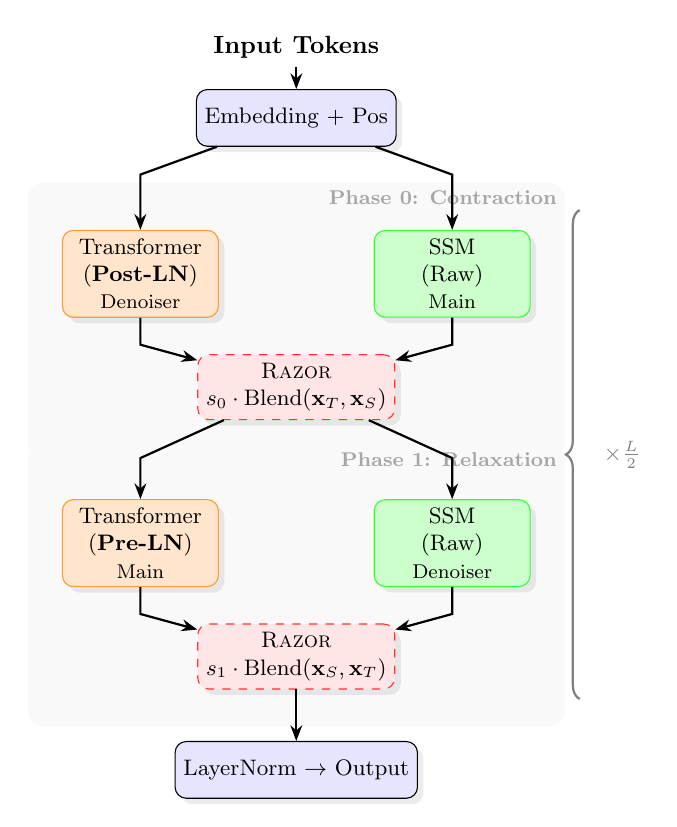
\begin{tikzpicture}[
    block/.style={draw, rounded corners, minimum width=2.2cm, minimum height=0.8cm, align=center, font=\small, drop shadow={opacity=0.15}},
    arrow/.style={-{Stealth[length=2mm]}, thick},
    phase/.style={fill=gray!5, rounded corners=6pt, inner sep=10pt},
    scale=0.9, transform shape
]
    % Phase backgrounds
    \node[phase, fit={(-3.4,-2.3) (3.4,-5.4)}] (even_phase) {};
    \node[anchor=north east, font=\footnotesize\bfseries\color{gray!70}] at (even_phase.north east) {Phase 0: Contraction};

    \node[phase, fit={(-3.4,-6.0) (3.4,-9.2)}] (odd_phase) {};
    \node[anchor=north east, font=\footnotesize\bfseries\color{gray!70}] at (odd_phase.north east) {Phase 1: Relaxation};

    % Input
    \node (input) at (0, 0) {\textbf{Input Tokens}};
    \node[block, fill=blue!10] (emb) at (0, -1) {Embedding + Pos};
    \draw[arrow] (input) -- (emb);

    % --- EVEN LAYER ---
    \node[block, fill=orange!20, draw=orange!80] (trans_e) at (-2.2, -3.2) {Transformer\\(\textbf{Post-LN})\\{\footnotesize Denoiser}};
    \node[block, fill=green!20, draw=green!80] (ssm_e) at (2.2, -3.2) {SSM\\(Raw)\\{\footnotesize Main}};
    \node[block, fill=red!10, draw=red!80, dashed] (razor_e) at (0, -4.8) {\razor{}\\$s_0 \cdot \text{Blend}(\xT, \xS)$};

    \draw[arrow] (emb) -- (-2.2, -1.8) -- (trans_e);
    \draw[arrow] (emb) -- (2.2, -1.8) -- (ssm_e);
    \draw[arrow] (trans_e) -- (-2.2, -4.2) -- (razor_e);
    \draw[arrow] (ssm_e) -- (2.2, -4.2) -- (razor_e);

    % --- ODD LAYER ---
    \node[block, fill=orange!20, draw=orange!80] (trans_o) at (-2.2, -7.0) {Transformer\\(\textbf{Pre-LN})\\{\footnotesize Main}};
    \node[block, fill=green!20, draw=green!80] (ssm_o) at (2.2, -7.0) {SSM\\(Raw)\\{\footnotesize Denoiser}};
    \node[block, fill=red!10, draw=red!80, dashed] (razor_o) at (0, -8.6) {\razor{}\\$s_1 \cdot \text{Blend}(\xS, \xT)$};

    \draw[arrow] (razor_e) -- (-2.2, -5.8) -- (trans_o);
    \draw[arrow] (razor_e) -- (2.2, -5.8) -- (ssm_o);
    \draw[arrow] (trans_o) -- (-2.2, -8.0) -- (razor_o);
    \draw[arrow] (ssm_o) -- (2.2, -8.0) -- (razor_o);

    % Output
    \node[block, fill=blue!10] (out) at (0, -10.2) {LayerNorm $\to$ Output};
    \draw[arrow] (razor_o) -- (out);

    % Repeat annotation
    \draw[decorate, decoration={brace, amplitude=5pt, mirror}, thick, gray]
        (4.0, -2.3) -- (4.0, -9.2) node[midway, right=6pt, font=\small, text=gray] {$\times \frac{L}{2}$};

\end{tikzpicture}
\caption{\altamba{} architecture illustrating the \textbf{Peristaltic Normalization} cycle. The ``Contraction'' phase (even layers) uses Post-LN for variance clamping, enabling precise destructive interference. The ``Relaxation'' phase (odd layers) uses Pre-LN for gradient flow, enabling constructive blending. Roles alternate: Transformer and SSM swap between main and denoiser each layer.}
\label{fig:architecture}
\end{figure}

\subsection{The \razor{} Blending Operation}
\label{sec:razor}

The \razor{} (formally, DualRazorNorm) is a parameterized blending module placed after each layer's dual-path computation. For layer $i$:

\textbf{Even layers} (Post-LN denoising, SSM main):
\begin{equation}
\label{eq:razor_even}
\mathbf{y}_i = s_0^{(i)} \cdot \Big[\underbrace{(1.4 - W_1^{(i)})}_{\alpha_d} \cdot \layernorm_d(\xT) + \underbrace{(0.6 - W_2^{(i)})}_{\alpha_m} \cdot \xS\Big]
\end{equation}

\textbf{Odd layers} (Pre-LN blending, Transformer main):
\begin{equation}
\label{eq:razor_odd}
\mathbf{y}_i = s_1^{(i)} \cdot \Big[\underbrace{(1.1 - W_1^{(i)})}_{\alpha_d} \cdot \layernorm_d(\xS) + \underbrace{(0.5 - W_2^{(i)})}_{\alpha_m} \cdot \xT\Big]
\end{equation}

where $W_1^{(i)}, W_2^{(i)} \in \R$ are learned scalars, $s_0^{(i)}$ and $s_1^{(i)}$ are learned output scales initialized to $+1.5$ and $-1.0$ respectively, and $\layernorm_d$ is a dedicated LayerNorm for the denoiser path.

The parameterization $(c - W)$ rather than a direct weight $\alpha$ provides several benefits:
\begin{enumerate}[nosep]
    \item The constants $c_1, c_2$ encode an \emph{inductive bias} for the initial blending strategy while allowing full flexibility through learning.
    \item The sign of the effective coefficient $\alpha = c - W$ determines whether the signal undergoes constructive ($\alpha > 0$) or destructive ($\alpha < 0$) interference.
    \item At initialization ($W_1 = 1.5, W_2 = -0.5$), even layers begin with aggressive SSM amplification ($+1.1\times$) and Transformer denoising ($-0.1\times$).
\end{enumerate}

\subsection{Peristaltic Normalization}
\label{sec:peristaltic}

The central architectural innovation is the \emph{alternating normalization pattern} applied to the Transformer path:

\begin{itemize}[nosep]
    \item \textbf{Even layers use Post-LN:} After multi-head attention, the output is residual-added and \emph{then} normalized. This clamps variance to approximately 1.0, creating a predictable signal for the \razor{}'s subtraction coefficient. The denoiser must be stable for precise interference.
    \item \textbf{Odd layers use Pre-LN:} Standard Pre-LN architecture where normalization occurs \emph{before} the sublayer. The residual stream preserves variance flexibility, enabling gradient flow and constructive feature growth.
\end{itemize}

This solves the historical gradient vanishing problem of pure Post-LN networks: Pre-LN layers act as ``repeater stations'' that re-establish clean gradient paths every other layer. Meanwhile, Post-LN layers provide the variance clamping necessary for precise destructive interference.

\textbf{Even-layer Transformer (Post-LN):}
\begin{align}
    \mathbf{h} &= \mathbf{x} + \text{MHA}(\mathbf{x}, \mathbf{x}, \mathbf{x}) \\
    \mathbf{h} &= \layernorm_1(\mathbf{h}) \\
    \xT &= \mathbf{h} + \text{FFN}(\layernorm_2(\mathbf{h}))
\end{align}

\textbf{Odd-layer Transformer (Pre-LN):}
\begin{align}
    \mathbf{h} &= \mathbf{x} + \text{MHA}(\layernorm_1(\mathbf{x})) \\
    \xT &= \mathbf{h} + \text{FFN}(\layernorm_2(\mathbf{h}))
\end{align}

\subsection{SSM Path}
\label{sec:ssm}

The SSM path uses Mamba-2~\cite{dao2024transformers} with native CUDA kernels for hardware efficiency. Each SSM block consists of:
\begin{equation}
    \xS = \mathbf{x} + \text{Dropout}(\layernorm(\text{Mamba2}(\mathbf{x})))
\end{equation}

We identify a previously undocumented instability in Mamba-2 when used in dual-path feedback architectures: the default unbounded \texttt{softplus} activation on the discretization timestep $\Delta$ allows values to grow without limit during training, driving the SSM into numerically unstable regimes. We address this with a bounded sigmoid reparameterization:
\begin{equation}
\label{eq:dt_bound}
    \Delta = \Delta_{\min} + (\Delta_{\max} - \Delta_{\min}) \cdot \sigma(\Delta_{\text{raw}})
\end{equation}
with $\Delta_{\min} = 0.001$ and $\Delta_{\max} = 0.1$, ensuring stable integration steps throughout training. Critically, we achieve this by computing $\Delta$ externally and passing it to the \texttt{mamba-ssm} kernel with \texttt{dt\_softplus=False}, preserving full CUDA hardware acceleration with no performance penalty. With $\Delta$ bounded to $[0.001, 0.1]$, the maximum approximation error of the simplified Euler discretization used internally by the kernel (i.e., $\bar{\mathbf{B}} = \Delta \mathbf{B}$ rather than the exact ZOH formula $\bar{\mathbf{B}} = (e^{\Delta \mathbf{A}} - \mathbf{I})\mathbf{A}^{-1}\mathbf{B}$) is below 1\%, rendering the approximation acceptable. The consequences of this fix for architectural interpretability are discussed in \S\ref{sec:vestigial}.

\subsection{Bottleneck Compression}
\label{sec:bottleneck}

The denoiser path operates at reduced dimensionality ($0.75\times$ of $d_{\text{model}}$) to improve parameter efficiency. For a model with $d_{\text{model}} = 2560$, the denoiser operates at 1920 dimensions. A learned linear projection maps the denoiser output back to $d_{\text{model}}$ before blending:
\begin{equation}
    \mathbf{x}_{\text{denoiser}}' = \mathbf{W}_{\text{proj}} \cdot \layernorm_d(\mathbf{x}_{\text{denoiser}}) + \mathbf{b}_{\text{proj}}, \quad \mathbf{W}_{\text{proj}} \in \R^{d_{\text{model}} \times d_{\text{denoiser}}}
\end{equation}

This compression provides two benefits: (1) parameter savings---the denoiser need not be as expressive as the main path; and (2) information bottleneck---forcing the denoiser to compress its representation may improve its noise-extraction capability.

\subsection{Output Scaling and Phase Alternation}
\label{sec:phase}

The learned output scales $s_0, s_1$ are initialized with alternating signs: $s_0 = +1.5$ for even layers, $s_1 = -1.0$ for odd layers. This creates a \emph{phase alternation} pattern where odd-layer outputs are sign-inverted relative to even-layer outputs.

At initialization, the effective operation of each layer type is:

\textbf{Even layers} (after $s_0 = +1.5$):
\begin{equation}
    \mathbf{y}_{\text{even}} \approx -0.15 \cdot \layernorm(\xT) + 1.65 \cdot \xS
\end{equation}

\textbf{Odd layers} (after $s_1 = -1.0$):
\begin{equation}
    \mathbf{y}_{\text{odd}} \approx +0.4 \cdot \layernorm(\xS) - 1.0 \cdot \xT
\end{equation}

The sign flip on odd layers means that both layer types contribute to a push-pull dynamic: even layers amplify the SSM while subtracting Transformer noise, and odd layers (after inversion) effectively subtract the Transformer main while adding normalized SSM corrections. The network learns to adjust $s_0, s_1$ away from these initializations as needed.

% ============================================================
\section{Experimental Setup}
\label{sec:experiments}
% ============================================================

\subsection{Dataset}

We train on the \textbf{Common Pile}~\cite{commonpile2025} (arXiv papers subset), consisting of full-length technical papers with dense mathematical notation, LaTeX formatting, and complex structured content. Tokenization uses the GPT-4 tokenizer (\texttt{cl100k\_base}) with vocabulary size 100{,}288 (padded to a multiple of 64 for hardware efficiency).

The dataset contains approximately 8M training tokens and 768K validation tokens, loaded in streaming chunks with periodic reloading to expose the model to diverse content throughout training.

\subsection{Model Configurations}

We evaluate \altamba{} at three parameter scales, each compared against a parameter-matched Jamba baseline (1:7 attention-to-Mamba ratio). \Cref{tab:configs} summarizes the configurations.

\begin{table}[t]
\centering
\caption{Model configurations across three scales. Baseline $d_{\text{model}}$ is adjusted via binary search to match \altamba{} parameter count within 1\%.}
\label{tab:configs}
\begin{tabular}{@{}lccc@{}}
\toprule
& \textbf{402M} & \textbf{1.08B} & \textbf{1.78B} \\
\midrule
\altamba{} $d_{\text{model}}$ & 1024 & 1536 & 2560 \\
Baseline $d_{\text{model}}$ & 1376 & --- & 2368 \\
Layers & 10 & 12 & 12 \\
Attention heads & 8 & 8 & 8 \\
FFN expansion & $4\times$ & $4\times$ & $4\times$ \\
Denoiser scale & $1.0\times$ & $1.0\times$ & $0.75\times$ \\
Denoiser $d$ & 1024 & 1536 & 1920 \\
Context length & 256 & 256 & 256 \\
\altamba{} params & 402M & 1.08B & 1779M \\
Baseline params & 401M & --- & 1766M \\
Param match & 0.20\% & --- & 0.74\% \\
\bottomrule
\end{tabular}
\end{table}

\subsection{Training}

All models are trained with AdamW~\cite{loshchilov2019decoupled} using the configuration in \cref{tab:training}.

\begin{table}[t]
\centering
\caption{Training hyperparameters (shared across all scales unless noted).}
\label{tab:training}
\begin{tabular}{@{}ll@{}}
\toprule
\textbf{Hyperparameter} & \textbf{Value} \\
\midrule
Batch size & 8 \\
Gradient accumulation & 8 steps \\
Effective batch size & 64 \\
Learning rate & $1 \times 10^{-4}$ \\
LR schedule & Cosine annealing ($\eta_{\min} = 0.1 \times \eta$) \\
Optimizer & AdamW \\
Mixed precision & BF16 \\
Gradient clipping & 1.0 \\
Dropout & 0.2 \\
Max training steps & 15{,}000 \\
\bottomrule
\end{tabular}
\end{table}

\textbf{Hardware.} The 402M experiments were conducted on an NVIDIA A40 (44.4\,GB). The 1.78B experiments use an NVIDIA RTX PRO 6000 Blackwell Server Edition (95\,GB). Gradient checkpointing is enabled for the Jamba baseline to fit within memory.

\subsection{Initialization Strategy}
\label{sec:init}

The \razor{} parameters are initialized as:
\begin{itemize}[nosep]
    \item $W_1 = 1.5$, $W_2 = -0.5$ for all layers
    \item $s_0 = +1.5$ (even layers), $s_1 = -1.0$ (odd layers)
\end{itemize}

This creates the following initial effective coefficients:

\textbf{Even layers} (SSM main, Transformer denoiser):
\begin{itemize}[nosep]
    \item Denoiser: $(1.4 - 1.5) \times 1.5 = -0.15$ (weak subtraction)
    \item Main: $(0.6 - (-0.5)) \times 1.5 = +1.65$ (strong amplification)
\end{itemize}

\textbf{Odd layers} (Transformer main, SSM denoiser):
\begin{itemize}[nosep]
    \item Denoiser: $(1.1 - 1.5) \times (-1.0) = +0.40$ (sign flip inverts subtraction into addition)
    \item Main: $(0.5 - (-0.5)) \times (-1.0) = -1.00$ (sign flip inverts the Transformer signal)
\end{itemize}

The negative output scale $s_1 = -1.0$ on odd layers naturally inverts the Transformer's contribution, creating a subtractive baseline: the \razor{} subtracts the Transformer signal while adding a normalized SSM correction. Combined with even layers that amplify SSM and subtract Transformer, this produces a consistent push-pull dynamic across the full network. The optimizer refines these initial coefficients per-layer during training.

% ============================================================
\section{Results}
\label{sec:results}
% ============================================================

\subsection{Performance Comparison}

\Cref{tab:results} presents validation loss results across scales. \altamba{} consistently outperforms the parameter-matched Jamba baseline at all scales tested.

\begin{table}[t]
\centering
\caption{Validation loss comparison. Improvement computed as $(\mathcal{L}_{\text{base}} - \mathcal{L}_{\text{ours}}) / \mathcal{L}_{\text{base}} \times 100\%$.}
\label{tab:results}
\begin{tabular}{@{}lcccr@{}}
\toprule
\textbf{Scale} & \textbf{Baseline Val} & \textbf{\altamba{} Val} & \textbf{Step} & \textbf{Improvement} \\
\midrule
402M & 3.1866 & 2.8886 & 1520 & 9.35\% \\
1.08B & 2.9771 & 2.6974 & 3580 & 9.40\% \\
1.78B & 2.4427 & 2.2554 & 8625 & 7.66\% \\
\bottomrule
\end{tabular}
\end{table}

At 402M and 1.08B parameters, \altamba{} achieves approximately 9.4\% improvement over parameter-matched baselines. At 1.78B, the model reaches a val loss of 2.26 with 7.66\% improvement at step 8625, approaching the gains seen at smaller scales. The absolute val loss (2.26) is substantially better than the 1.08B peak (2.70). Throughout training, the \altamba{} model maintains a healthier train-val gap (0.18 vs 0.29 for the baseline at step 8625), suggesting the dual-path architecture provides implicit regularization.

\subsection{Normalization Strategy Ablation}

During development, we explored several normalization configurations for the dual-path architecture (\cref{tab:ablation}). The progression reveals that normalization choice is critical:

\begin{table}[t]
\centering
\caption{Normalization strategy ablation (402M scale). All configurations use the same \razor{} blending with identical $W$ initialization.}
\label{tab:ablation}
\begin{tabular}{@{}llr@{}}
\toprule
\textbf{Configuration} & \textbf{Description} & \textbf{Improvement} \\
\midrule
Traditional & Post-LN everywhere, Transformer main & 9.0\% \\
Reversed & Pre-LN everywhere, SSM main & 10.63\% \\
Hybrid & Post-LN attention + Pre-LN FFN & 11.93\% \\
Peristaltic & Alternating Post/Pre + role reversal & 11.3\%+ \\
\bottomrule
\end{tabular}
\end{table}

The ``Reversed'' configuration---making SSM the main signal carrier instead of Transformer---provided a substantial jump from 9.0\% to 10.63\%, suggesting that SSMs benefit more from the denoising treatment. The hybrid and peristaltic configurations push further by exploiting normalization diversity.

\subsection{Learned Weight Analysis (1.78B Scale)}
\label{sec:weights_1b8}

\Cref{tab:weights} shows the per-layer learned $W_1, W_2$ values at convergence (step 8625) of the 1.78B run. Several patterns emerge.

\begin{table}[t]
\centering
\caption{Per-layer learned \razor{} weights at convergence (1.78B, step 8625). Effective coefficients computed as $\alpha_d = c_1 - W_1$ (denoiser) and $\alpha_m = c_2 - W_2$ (main), \emph{before} output scaling.}
\label{tab:weights}
\begin{tabular}{@{}crrrrrl@{}}
\toprule
\textbf{Layer} & $W_1$ & $W_2$ & $\alpha_d$ & $\alpha_m$ & $s$ & \textbf{Role} \\
\midrule
0 & $+1.537$ & $-0.272$ & $-0.137$ & $+0.872$ & $+1.5$ & Even: SSM main \\
1 & $+1.596$ & $-0.295$ & $-0.496$ & $+0.795$ & $-1.0$ & Odd: Trans main \\
2 & $+1.422$ & $-0.313$ & $-0.022$ & $+0.913$ & $+1.5$ & Even: SSM main \\
3 & $+1.491$ & $-0.386$ & $-0.391$ & $+0.886$ & $-1.0$ & Odd: Trans main \\
4 & $+1.408$ & $-0.289$ & $-0.008$ & $+0.889$ & $+1.5$ & Even: SSM main \\
5 & $+1.511$ & $-0.415$ & $-0.411$ & $+0.915$ & $-1.0$ & Odd: Trans main \\
6 & $+1.404$ & $-0.343$ & $-0.004$ & $+0.943$ & $+1.5$ & Even: SSM main \\
7 & $+1.421$ & $-0.427$ & $-0.321$ & $+0.927$ & $-1.0$ & Odd: Trans main \\
8 & $+1.443$ & $-0.425$ & $-0.043$ & $+1.025$ & $+1.5$ & Even: SSM main \\
9 & $+1.407$ & $-0.430$ & $-0.307$ & $+0.930$ & $-1.0$ & Odd: Trans main \\
10 & $+1.472$ & $-0.530$ & $-0.072$ & $+1.130$ & $+1.5$ & Even: SSM main \\
11 & $+1.514$ & $-0.472$ & $-0.414$ & $+0.972$ & $-1.0$ & Odd: Trans main \\
\bottomrule
\end{tabular}
\end{table}

\begin{figure}[t]
\centering
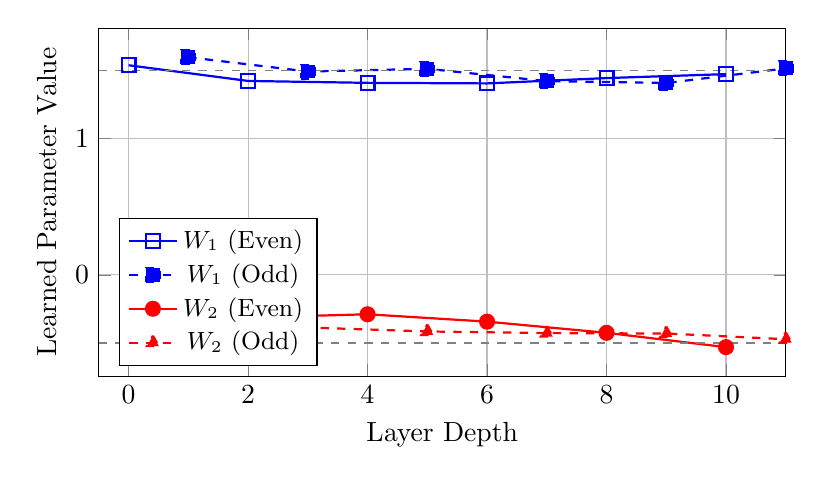
\begin{tikzpicture}
\begin{axis}[
    xlabel={Layer Depth},
    ylabel={Learned Parameter Value},
    grid=major,
    legend pos=south west,
    width=0.85\textwidth,
    height=6cm,
    xtick={0,2,4,6,8,10},
    xmin=-0.5, xmax=11,
    legend style={font=\small},
    every axis plot/.append style={thick}
]
% W1 (Even Layers) - relatively flat
\addplot[color=blue, mark=square, mark size=2.5pt] coordinates {
    (0, 1.537) (2, 1.422) (4, 1.408) (6, 1.404) (8, 1.443) (10, 1.472)
};
\addlegendentry{$W_1$ (Even)}

% W1 (Odd Layers)
\addplot[color=blue, mark=square*, mark size=2.5pt, dashed] coordinates {
    (1, 1.596) (3, 1.491) (5, 1.511) (7, 1.421) (9, 1.407) (11, 1.514)
};
\addlegendentry{$W_1$ (Odd)}

% W2 (Even Layers) - trending more negative with depth
\addplot[color=red, mark=*, mark size=2.5pt] coordinates {
    (0, -0.272) (2, -0.313) (4, -0.289) (6, -0.343) (8, -0.425) (10, -0.530)
};
\addlegendentry{$W_2$ (Even)}

% W2 (Odd Layers)
\addplot[color=red, mark=triangle*, mark size=2.5pt, dashed] coordinates {
    (1, -0.295) (3, -0.386) (5, -0.415) (7, -0.427) (9, -0.430) (11, -0.472)
};
\addlegendentry{$W_2$ (Odd)}

% Reference lines
\draw[gray, thin, dashed] (axis cs:-0.5,1.5) -- (axis cs:11,1.5) node[right, font=\tiny] {$W_1$ init};
\draw[gray, thin, dashed] (axis cs:-0.5,-0.5) -- (axis cs:11,-0.5) node[right, font=\tiny] {$W_2$ init};
\end{axis}
\end{tikzpicture}
\caption{Evolution of \razor{} parameters across depth (1.78B, step 8625). $W_1$ remains near initialization ($1.5$, dashed gray), indicating the denoiser coefficient is architecturally determined. $W_2$ trends downward with depth---deeper layers amplify the main signal more aggressively, consistent with depth-dependent denoising.}
\label{fig:weights_plot}
\end{figure}

\begin{figure}[t]
\centering
\includegraphics[width=\textwidth]{figures/razor_parameters.pdf}
\caption{Three-stage view of learned \razor{} parameters (1.78B, step 8100 checkpoint). \textbf{Left:} Raw $W_1, W_2$ values with initialization references. \textbf{Center:} Effective pre-scaling coefficients $\alpha_d = c - W_1$ (denoiser) and $\alpha_m = c' - W_2$ (main). The denoiser coefficients are consistently small and negative, while main coefficients cluster near 1.0. \textbf{Right:} Post-scaling coefficients $\alpha^* = s \cdot \alpha$, revealing the push-pull dynamic: even layers (blue) amplify the main path ($\alpha_m^* > 0$), odd layers (orange) invert it ($\alpha_m^* < 0$). The depth gradient in $\alpha_m^*$ is clearly visible, with deeper even layers reaching $+1.7\times$ main amplification.}
\label{fig:razor_panels}
\end{figure}

\textbf{Observation 1: Depth-dependent denoising.} $W_2$ becomes more negative in deeper layers ($-0.313$ at layer 2 $\to$ $-0.530$ at layer 10), increasing the effective main-signal coefficient $\alpha_m$. This means deeper layers amplify the main signal more aggressively. Intuitively, this corresponds to error accumulation through depth requiring progressively stronger correction. The depth gradient steepens throughout training: the $W_2$ spread between layer 0 and layer 10 grew from $0.147$ (step 1900) to $0.258$ (step 8625), as early layers relax (layer 0: $-0.386 \to -0.272$) while deeper layers hold firm (layer 10: $-0.533 \to -0.530$).

\textbf{Observation 2: Near-identity main path.} The effective main coefficient $\alpha_m$ clusters around 1.0 across all layers (range: 0.795--1.130 before scaling), indicating the model converges toward a near-identity residual stream for the main path with small denoiser corrections---analogous to ResNet-style skip connections with learned perturbations.

\textbf{Observation 3: Weak denoiser corrections.} The denoiser coefficients $\alpha_d$ are small in magnitude (even layers: $-0.14$ to $-0.00$; odd layers: $-0.31$ to $-0.50$), confirming the hypothesis that the denoiser performs \emph{small surgical corrections} rather than large-scale signal transformation. Notably, even-layer denoiser coefficients in the middle layers (4, 6) approach zero ($\alpha_d \approx -0.01$), suggesting these layers rely almost entirely on the main SSM path.

\textbf{Observation 4: Asymmetric parameter adaptation.} $W_1$ drifts slowly from initialization (avg 1.469 vs init 1.500), while $W_2$ shows substantially more movement (avg $-0.383$ vs init $-0.500$). The optimizer primarily adjusts the main-signal coefficient rather than the denoiser coefficient, suggesting the denoiser's role is structurally determined by the architecture (normalization choice, bottleneck) while the main-path gain requires per-layer tuning.

% ============================================================
\section{Analysis}
\label{sec:analysis}
% ============================================================

\subsection{Effective Layer Operations After Scaling}

Accounting for the output scales $s_0 = +1.5$ and $s_1 = -1.0$, the effective per-layer operations at convergence (step 8625, using average weights) are:

\textbf{Even layers:}
\begin{equation}
    \mathbf{y}_{\text{even}} = 1.5 \times \Big[-0.05 \cdot \layernorm(\xT) + 0.96 \cdot \xS\Big] \approx -0.07 \cdot \layernorm(\xT) + 1.44 \cdot \xS
\end{equation}

\textbf{Odd layers:}
\begin{equation}
    \mathbf{y}_{\text{odd}} = (-1.0) \times \Big[-0.39 \cdot \layernorm(\xS) + 0.90 \cdot \xT\Big] \approx +0.39 \cdot \layernorm(\xS) - 0.90 \cdot \xT
\end{equation}

The sign inversion on odd layers means that both layer types contribute to a consistent pattern: \emph{amplify SSM-derived signal, subtract or attenuate Transformer signal}. Even layers do this directly ($+1.44 \times$ SSM, $-0.07 \times$ Trans); odd layers do this through sign inversion ($+0.39 \times$ SSM, $-0.90 \times$ Trans). The SSM is the preferred signal carrier throughout the network. Compared to early training, the even-layer coefficients have relaxed (main amplification decreased from $1.55\times$ to $1.44\times$), consistent with the model needing less aggressive correction as representations mature.

\subsection{Three-Stage Gain Staging}

At larger scales (1.08B), the learned weights exhibit a three-stage pattern analogous to professional audio signal chains:

\begin{enumerate}[nosep]
    \item \textbf{Pre-Amp (Layers 0--1):} Elevated energy injection ($+15\%$ above baseline), establishing initial signal strength.
    \item \textbf{Linear Middle (Layers 2--4):} Minimal gain adjustment, clean signal propagation at approximately $128.7\%$ energy.
    \item \textbf{Limiter (Layer 9+):} Maximum compression/braking ($156.2\%$ energy cap), preventing saturation before the output projection.
\end{enumerate}

This emergent gain staging was not engineered but discovered by the optimizer, suggesting that signal-level management across depth is a fundamental requirement that the architecture's flexible parameterization allows the model to learn.

\subsection{Stability Analysis: The Vestigial Organ Phenomenon}
\label{sec:vestigial}

In early experiments at 1.08B scale (prior to the bounded-$\Delta$ fix of \S\ref{sec:ssm}), layers 5, 7, and 9 converged to $W_1 \approx 1.5$, effectively zeroing the SSM denoiser contribution on odd layers. We initially interpreted this as a structural redundancy signal---a ``vestigial organ''---and implemented a sparse variant (ALTAMBA-Sparse) that pruned SSM blocks from these layers for approximately $15\%$ FLOPs savings.

This interpretation was incorrect. The behavior was a \emph{stability artifact}: with unbounded \texttt{softplus} activation on the discretization timestep $\Delta$, values of $\Delta$ could grow without limit during training, driving the SSM into numerically unstable regimes. The optimizer compensated by learning to shut off the unstable path entirely via $W_1 \to 1.5$. Once $\Delta$ was bounded to $[\Delta_{\min}, \Delta_{\max}]$ via sigmoid (\cref{eq:dt_bound}), the SSM path remained stable and the denoiser on odd layers contributed meaningfully at all depths (see \cref{tab:weights}: all odd-layer $|\alpha_d| \in [0.307, 0.496]$).

This finding carries a broader lesson for interpretability of learned architecture parameters: \emph{learned weight patterns may reflect optimization artifacts rather than genuine architectural insights}. What appeared to be the network discovering redundancy was in fact the network protecting itself from a numerically unstable component. We recommend that any ``architecture search via learned coefficients'' approach verify findings under different numerical conditioning before drawing structural conclusions.

\subsection{Gradient Flow Analysis}

A potential concern with Post-LN layers is gradient vanishing. \altamba{} mitigates this through two mechanisms:

\begin{enumerate}[nosep]
    \item \textbf{Parallel SSM highway (even layers):} Even when the Transformer path uses Post-LN, the parallel SSM path provides an ungated gradient highway through the Mamba-2 blocks.
    \item \textbf{Pre-LN alternation (odd layers):} Every other layer uses standard Pre-LN with full residual connections, re-establishing clean gradient flow.
\end{enumerate}

The result is that no gradient must traverse more than one Post-LN layer without encountering a gradient-friendly Pre-LN layer, preventing the cascading attenuation that plagues pure Post-LN networks.

\subsection{Weight Magnitude Analysis}
\label{sec:weight_magnitudes}

\Cref{fig:weight_norms} shows Frobenius norms of the major weight matrices across all 12 layers, revealing that role alternation is reflected not only in the learned \razor{} coefficients but in the weight magnitudes themselves. Even-layer Transformer weights (denoiser role, 1920 dimensions) have consistently smaller norms ($\sim$56 for attention in-projection) than odd-layer Transformer weights (main role, 2560 dimensions, $\sim$67--69). SSM norms show the inverse pattern: even-layer SSM in-projection norms ($\sim$69--72) exceed odd-layer norms ($\sim$54--62), consistent with the SSM carrying the main signal on even layers.

The alternating ``checkerboard'' pattern in \cref{fig:weight_norms} provides independent confirmation that the two paths specialize for their assigned roles. Notably, the SSM in-projection norms increase with depth on even layers (69 at layer 0 $\to$ 72 at layers 8--10), paralleling the depth-dependent $W_2$ trend observed in the \razor{} parameters (\cref{fig:weights_plot}).

\begin{figure}[t]
\centering
\includegraphics[width=\textwidth]{figures/weight_norm_heatmap.pdf}
\caption{Frobenius norms of weight matrices across layers (1.78B, step 8100 checkpoint). Each cell shows the absolute norm; color is column-normalized. The alternating pattern confirms that role assignment (main vs.\ denoiser) is reflected in weight magnitudes: main-role weights are consistently larger than denoiser-role weights for both Transformer and SSM paths.}
\label{fig:weight_norms}
\end{figure}

\subsection{Spectral Analysis of Attention Weights}
\label{sec:spectral}

To understand how the Transformer path adapts to its dual roles, we compute the singular value decomposition of the attention in-projection weights $\mathbf{W}_{\text{in}} \in \R^{3d \times d}$ for each layer (\cref{fig:sv_spectra}).

Even-layer attention (denoiser role, $d = 1920$) develops \emph{steep spectral decay}: normalized singular values drop to $\sim$0.15 by index 100, indicating the attention operates as a low-rank projection. This is consistent with the denoiser performing targeted, low-dimensional corrections rather than full-rank transformations. In contrast, odd-layer attention (main role, $d = 2560$) maintains \emph{flat spectra} with singular values staying above $\sim$0.5, indicating near-full-rank utilization of the available capacity.

This spectral bifurcation emerges entirely from training---both paths are initialized identically (up to dimension scaling). The denoiser attention learns that it needs only a few principal directions to extract useful corrections, while the main attention requires broad representational capacity. This finding further supports the architectural choice of bottleneck compression ($0.75\times$) for the denoiser: the denoiser does not use its full capacity even at the reduced dimension.

\begin{figure}[t]
\centering
\includegraphics[width=\textwidth]{figures/singular_values_attention.pdf}
\caption{Normalized singular value spectra of attention in-projection weights. \textbf{Left:} Even layers (Transformer = denoiser, 1920d) show steep decay, indicating low-rank structure. \textbf{Right:} Odd layers (Transformer = main, 2560d) maintain flat spectra, using near-full rank. The spectral gap confirms that the denoiser performs surgical, low-dimensional corrections.}
\label{fig:sv_spectra}
\end{figure}

\subsection{SSM Parameter Analysis}
\label{sec:ssm_analysis}

\Cref{fig:ssm_params} examines the internal Mamba-2 parameters across layers. The decay rates $\exp(A_{\log})$ control how quickly the SSM's hidden state forgets past inputs. Values are broadly similar across roles (median $\sim$8 for both even and odd layers), suggesting the SSM's temporal dynamics are not strongly differentiated by role assignment. However, the $D$ parameter (direct skip connection from input to output) shows a subtle depth trend: deeper odd-layer (denoiser) SSMs reduce their skip connection strength toward 0.95--0.98, suggesting these layers increasingly rely on recurrent processing rather than direct passthrough.

\Cref{fig:dt_bias} shows the learned discretization timestep biases $\Delta_{\text{bias}}$, which are added to raw $\Delta$ values before the bounded sigmoid (\cref{eq:dt_bound}). All biases are strongly negative ($-3$ to $-7$), pushing $\sigma(\Delta_{\text{raw}} + \Delta_{\text{bias}})$ toward zero and keeping effective $\Delta$ near $\Delta_{\min} = 0.001$. This confirms that the bounded-$\Delta$ fix is actively utilized: the model prefers small integration steps throughout, consistent with precise state updates. Even-layer SSMs (main role, 80 heads) show wider bias distributions than odd-layer SSMs (denoiser role, 60 heads), suggesting the main-path SSM maintains more diverse temporal resolution across its heads.

\begin{figure}[t]
\centering
\includegraphics[width=\textwidth]{figures/ssm_parameters.pdf}
\caption{Mamba-2 internal parameters across layers (1.78B, step 8100 checkpoint). \textbf{Left:} Decay rates $\exp(A_{\log})$ are similar across roles, indicating temporal dynamics are not strongly differentiated by main vs.\ denoiser assignment. \textbf{Right:} The $D$ skip connection parameter shows deeper denoiser layers (odd, orange) slightly reducing skip strength, favoring recurrent processing.}
\label{fig:ssm_params}
\end{figure}

\begin{figure}[t]
\centering
\includegraphics[width=\textwidth]{figures/dt_bias_distribution.pdf}
\caption{Learned discretization timestep bias $\Delta_{\text{bias}}$ per layer (1.78B, step 8100 checkpoint). Strongly negative biases push $\sigma(\Delta_{\text{raw}} + \Delta_{\text{bias}})$ toward zero, keeping effective $\Delta \approx \Delta_{\min}$. Even-layer SSMs (main, blue, 80 heads) maintain wider distributions than odd-layer SSMs (denoiser, orange, 60 heads).}
\label{fig:dt_bias}
\end{figure}

% ============================================================
\section{Related Work}
\label{sec:related}
% ============================================================

\textbf{Normalization strategies.} Post-LN was introduced in the original Transformer~\cite{vaswani2017attention} and used in BERT~\cite{devlin2019bert}. Pre-LN was adopted by GPT-2~\cite{radford2019language} for training stability and has since become universal. \citet{xiong2020layer} analyzed the gradient flow differences. RMSNorm~\cite{zhang2019root} simplifies LayerNorm by removing mean centering. Our work is the first to \emph{strategically alternate} Post-LN and Pre-LN within a single model for complementary computational roles.

\textbf{State Space Models.} S4~\cite{gu2022efficiently} introduced structured state spaces for long-range dependencies. Mamba~\cite{gu2023mamba} added input-dependent selectivity. Mamba-2~\cite{dao2024transformers} reformulated SSMs through structured state space duality. Our SSM path uses Mamba-2 with bounded-sigmoid $\Delta$ for numerical stability.

\textbf{Hybrid architectures.} Jamba~\cite{lieber2024jamba} interleaves Transformer and Mamba layers at a fixed 1:7 ratio. \altamba{} differs fundamentally: both paths operate \emph{in parallel} at every layer with learned blending, rather than serial interleaving with fixed allocation.

\textbf{Multi-path architectures.} Mixture-of-Experts~\cite{shazeer2017outrageously} routes tokens to different experts. Highway Networks~\cite{srivastava2015highway} use gated residual connections. Our approach differs in using two architecturally distinct paths (Transformer and SSM) with a learned interference operation rather than gating or routing.

\textbf{Signal processing in neural networks.} The connection between neural networks and signal processing has been explored through Fourier features~\cite{tancik2020fourier}, spectral normalization~\cite{miyato2018spectral}, and frequency-domain analysis of attention~\cite{wen2023frequencies}. Our destructive interference framing provides a new lens for understanding dual-path architectures.

% ============================================================
\section{Discussion}
\label{sec:discussion}
% ============================================================

\textbf{Why does normalization diversity help?} We hypothesize that Post-LN and Pre-LN induce fundamentally different representation geometries, and alternating between them gives the network access to complementary operations. Post-LN confines the residual stream to a compact manifold---a unit hypersphere ($\|\mathbf{x}\|_2 \approx \sqrt{d}$, zero mean)---where the \razor{} acts as a \emph{projection} operator, measuring and subtracting angular differences between signals. This geometric constraint is precisely what makes destructive interference reliable: subtraction on a hypersphere is well-conditioned regardless of input magnitude. Pre-LN, by contrast, preserves the ambient Euclidean geometry of the representation space, allowing the manifold to expand freely. Here the \razor{} acts as a \emph{translation} operator, composing features additively without variance constraints. By alternating between projection (Post-LN) and translation (Pre-LN), the network can perform precise noise subtraction and expressive feature growth in the layers where each is most effective.

\textbf{SSM as preferred signal carrier.} Across all experiments, the learned weights consistently amplify the SSM path and attenuate the Transformer path. This suggests that for the task of next-token prediction on technical text, the SSM's recurrent dynamics provide a better ``backbone'' signal than attention, with attention serving primarily as a noise-reduction mechanism---an inversion of the conventional wisdom.

\textbf{Limitations.}
\begin{itemize}[nosep]
    \item All experiments use a single domain (arXiv technical papers). Generalization to diverse corpora remains to be validated.
    \item The 1.78B run was trained to step 8625. Longer training may yield different dynamics.
    \item Context length is limited to 256 tokens. Behavior at longer contexts is unexplored.
    \item The bounded-$\Delta$ fix for Mamba-2 may limit the SSM's expressivity. The trade-off between stability and flexibility warrants further study.
    \item Computational overhead: running two full paths per layer approximately doubles per-layer FLOPs compared to a single-path model (partially offset by the 0.75$\times$ bottleneck).
\end{itemize}

\textbf{Future work.}
\begin{itemize}[nosep]
    \item Scaling to larger models and diverse datasets.
    \item Extending phase alternation patterns beyond $\pm$ scaling.
    \item Applying the peristaltic normalization principle to other dual-path architectures.
    \item Longer context lengths with efficient attention variants.
\end{itemize}

% ============================================================
\section{Conclusion}
\label{sec:conclusion}
% ============================================================

We introduced \altamba{}, a dual-path architecture that achieves consistent improvements over parameter-matched Jamba baselines through two key innovations: the \razor{} learnable blending operation and Peristaltic Normalization. By strategically alternating Post-LayerNorm (for precise destructive interference) and Pre-LayerNorm (for expressive constructive blending) with role reversal between layers, the architecture unlocks denoising capabilities that neither normalization alone can provide.

Across three scales (402M, 1.08B, 1.78B parameters), \altamba{} achieves 8--9\% validation loss improvements, with the learned weights revealing interpretable emergent behaviors: depth-dependent denoising strength and three-stage gain staging. These findings suggest that \emph{normalization diversity}---using different normalization strategies for different computational roles---is a powerful and underexplored design principle for deep networks.

The core lesson: Post-LayerNorm was abandoned because it failed as a \emph{universal} normalization. We show it excels as a \emph{specialized} tool for destructive interference, when alternated with Pre-LN layers that ensure gradient flow.

\paragraph{Code Availability.} Code and model checkpoints are available at \url{https://github.com/altamba/altamba}.

% ============================================================
% References
% ============================================================
\bibliographystyle{plainnat}

\begin{thebibliography}{99}

\bibitem[Brown et~al.(2020)]{brown2020language}
Tom Brown, Benjamin Mann, Nick Ryder, Melanie Subbiah, Jared~D Kaplan, et~al.
\newblock Language models are few-shot learners.
\newblock In \emph{NeurIPS}, 2020.

\bibitem[Dao \& Gu(2024)]{dao2024transformers}
Tri Dao and Albert Gu.
\newblock Transformers are {SSM}s: Generalized models and efficient algorithms through structured state space duality.
\newblock In \emph{ICML}, 2024.

\bibitem[Devlin et~al.(2019)]{devlin2019bert}
Jacob Devlin, Ming-Wei Chang, Kenton Lee, and Kristina Toutanova.
\newblock {BERT}: Pre-training of deep bidirectional transformers for language understanding.
\newblock In \emph{NAACL}, 2019.

\bibitem[Common Pile(2025)]{commonpile2025}
Common Pile.
\newblock Common {Pile} v0.1: Filtered and deduplicated pre-training data.
\newblock \url{https://huggingface.co/collections/common-pile/common-pile-v01-filtered-data}, 2025.

\bibitem[Gu et~al.(2022)]{gu2022efficiently}
Albert Gu, Karan Goel, and Christopher R\'{e}.
\newblock Efficiently modeling long sequences with structured state spaces.
\newblock In \emph{ICLR}, 2022.

\bibitem[Gu \& Dao(2023)]{gu2023mamba}
Albert Gu and Tri Dao.
\newblock Mamba: Linear-time sequence modeling with selective state spaces.
\newblock \emph{arXiv:2312.00752}, 2023.

\bibitem[Lieber et~al.(2024)]{lieber2024jamba}
Opher Lieber, Barak Lenz, Hofit Bata, Gal Cohen, Jhonathan Osin, et~al.
\newblock Jamba: A hybrid {T}ransformer-{M}amba language model.
\newblock \emph{arXiv:2403.19887}, 2024.

\bibitem[Loshchilov \& Hutter(2019)]{loshchilov2019decoupled}
Ilya Loshchilov and Frank Hutter.
\newblock Decoupled weight decay regularization.
\newblock In \emph{ICLR}, 2019.

\bibitem[Miyato et~al.(2018)]{miyato2018spectral}
Takeru Miyato, Toshiki Kataoka, Masanori Koyama, and Yuichi Yoshida.
\newblock Spectral normalization for generative adversarial networks.
\newblock In \emph{ICLR}, 2018.

\bibitem[Radford et~al.(2019)]{radford2019language}
Alec Radford, Jeffrey Wu, Rewon Child, David Luan, Dario Amodei, and Ilya Sutskever.
\newblock Language models are unsupervised multitask learners.
\newblock \emph{OpenAI Blog}, 2019.

\bibitem[Shazeer et~al.(2017)]{shazeer2017outrageously}
Noam Shazeer, Azalia Mirhoseini, Krzysztof Maziarz, Andy Davis, Quoc Le, Geoffrey Hinton, and Jeff Dean.
\newblock Outrageously large neural networks: The sparsely-gated mixture-of-experts layer.
\newblock In \emph{ICLR}, 2017.

\bibitem[Srivastava et~al.(2015)]{srivastava2015highway}
Rupesh~K Srivastava, Klaus Greff, and J\"{u}rgen Schmidhuber.
\newblock Highway networks.
\newblock \emph{arXiv:1505.00387}, 2015.

\bibitem[Tancik et~al.(2020)]{tancik2020fourier}
Matthew Tancik, Pratul Srinivasan, Ben Mildenhall, Sara Fridovich-Keil, Nithin Raghavan, et~al.
\newblock Fourier features let networks learn high frequency functions in low dimensional domains.
\newblock In \emph{NeurIPS}, 2020.

\bibitem[Touvron et~al.(2023)]{touvron2023llama}
Hugo Touvron, Thibaut Lavril, Gautier Izacard, Xavier Martinet, et~al.
\newblock {LLaMA}: Open and efficient foundation language models.
\newblock \emph{arXiv:2302.13971}, 2023.

\bibitem[Vaswani et~al.(2017)]{vaswani2017attention}
Ashish Vaswani, Noam Shazeer, Niki Parmar, Jakob Uszkoreit, Llion Jones, Aidan~N Gomez, {\L}ukasz Kaiser, and Illia Polosukhin.
\newblock Attention is all you need.
\newblock In \emph{NeurIPS}, 2017.

\bibitem[Wen et~al.(2023)]{wen2023frequencies}
Yiqun Wen, Dong Li, and Jian Sun.
\newblock On the frequencies of attention.
\newblock \emph{arXiv}, 2023.

\bibitem[Xiong et~al.(2020)]{xiong2020layer}
Ruibin Xiong, Yunchang Yang, Di~He, Kai Zheng, Shuxin Zheng, et~al.
\newblock On layer normalization in the transformer architecture.
\newblock In \emph{ICML}, 2020.

\bibitem[Zhang \& Sennrich(2019)]{zhang2019root}
Biao Zhang and Rico Sennrich.
\newblock Root mean square layer normalization.
\newblock In \emph{NeurIPS}, 2019.

\end{thebibliography}

% ============================================================
\appendix
\section{DualRazorNorm Implementation}
\label{app:implementation}
% ============================================================

\begin{algorithm}[h]
\caption{DualRazorNorm Forward Pass}
\label{alg:razor}
\begin{algorithmic}[1]
\REQUIRE Main signal $\mathbf{x}_m \in \R^{B \times T \times d}$, denoiser signal $\mathbf{x}_d \in \R^{B \times T \times d'}$, layer index $i$
\ENSURE Blended output $\mathbf{y} \in \R^{B \times T \times d}$
\STATE $\hat{\mathbf{x}}_d \gets \layernorm_d(\mathbf{x}_d)$
\IF{$d' \neq d$}
    \STATE $\hat{\mathbf{x}}_d \gets \mathbf{W}_{\text{proj}} \hat{\mathbf{x}}_d + \mathbf{b}_{\text{proj}}$ \COMMENT{Project denoiser to main dimension}
\ENDIF
\IF{$i \bmod 2 = 0$}
    \STATE $\mathbf{y} \gets (1.4 - W_1) \cdot \hat{\mathbf{x}}_d + (0.6 - W_2) \cdot \mathbf{x}_m$ \COMMENT{Even: Post-LN denoising}
    \STATE $\mathbf{y} \gets s_0 \cdot \mathbf{y}$
\ELSE
    \STATE $\mathbf{y} \gets (1.1 - W_1) \cdot \hat{\mathbf{x}}_d + (0.5 - W_2) \cdot \mathbf{x}_m$ \COMMENT{Odd: Pre-LN blending}
    \STATE $\mathbf{y} \gets s_1 \cdot \mathbf{y}$
\ENDIF
\RETURN $\mathbf{y}$
\end{algorithmic}
\end{algorithm}

\section{Full Per-Layer Analysis (1.78B, Step 8625)}
\label{app:full_weights}

\Cref{tab:full_weights} reports the complete effective coefficients after applying output scaling for all 12 layers at convergence.

\begin{table}[h]
\centering
\caption{Effective coefficients after output scaling (1.78B, step 8625). $\alpha_d^* = s \cdot (c_1 - W_1)$ and $\alpha_m^* = s \cdot (c_2 - W_2)$.}
\label{tab:full_weights}
\begin{tabular}{@{}crrrr@{}}
\toprule
\textbf{Layer} & $\alpha_d^*$ (Denoiser) & $\alpha_m^*$ (Main) & \textbf{Type} \\
\midrule
0 & $-0.206$ & $+1.308$ & Even (Post-LN) \\
1 & $+0.496$ & $-0.795$ & Odd (Pre-LN) \\
2 & $-0.033$ & $+1.370$ & Even (Post-LN) \\
3 & $+0.391$ & $-0.886$ & Odd (Pre-LN) \\
4 & $-0.012$ & $+1.334$ & Even (Post-LN) \\
5 & $+0.411$ & $-0.915$ & Odd (Pre-LN) \\
6 & $-0.006$ & $+1.415$ & Even (Post-LN) \\
7 & $+0.321$ & $-0.927$ & Odd (Pre-LN) \\
8 & $-0.065$ & $+1.538$ & Even (Post-LN) \\
9 & $+0.307$ & $-0.930$ & Odd (Pre-LN) \\
10 & $-0.108$ & $+1.695$ & Even (Post-LN) \\
11 & $+0.414$ & $-0.972$ & Odd (Pre-LN) \\
\bottomrule
\end{tabular}
\end{table}

\end{document}
